\begin{figure}[!htb]
\centering
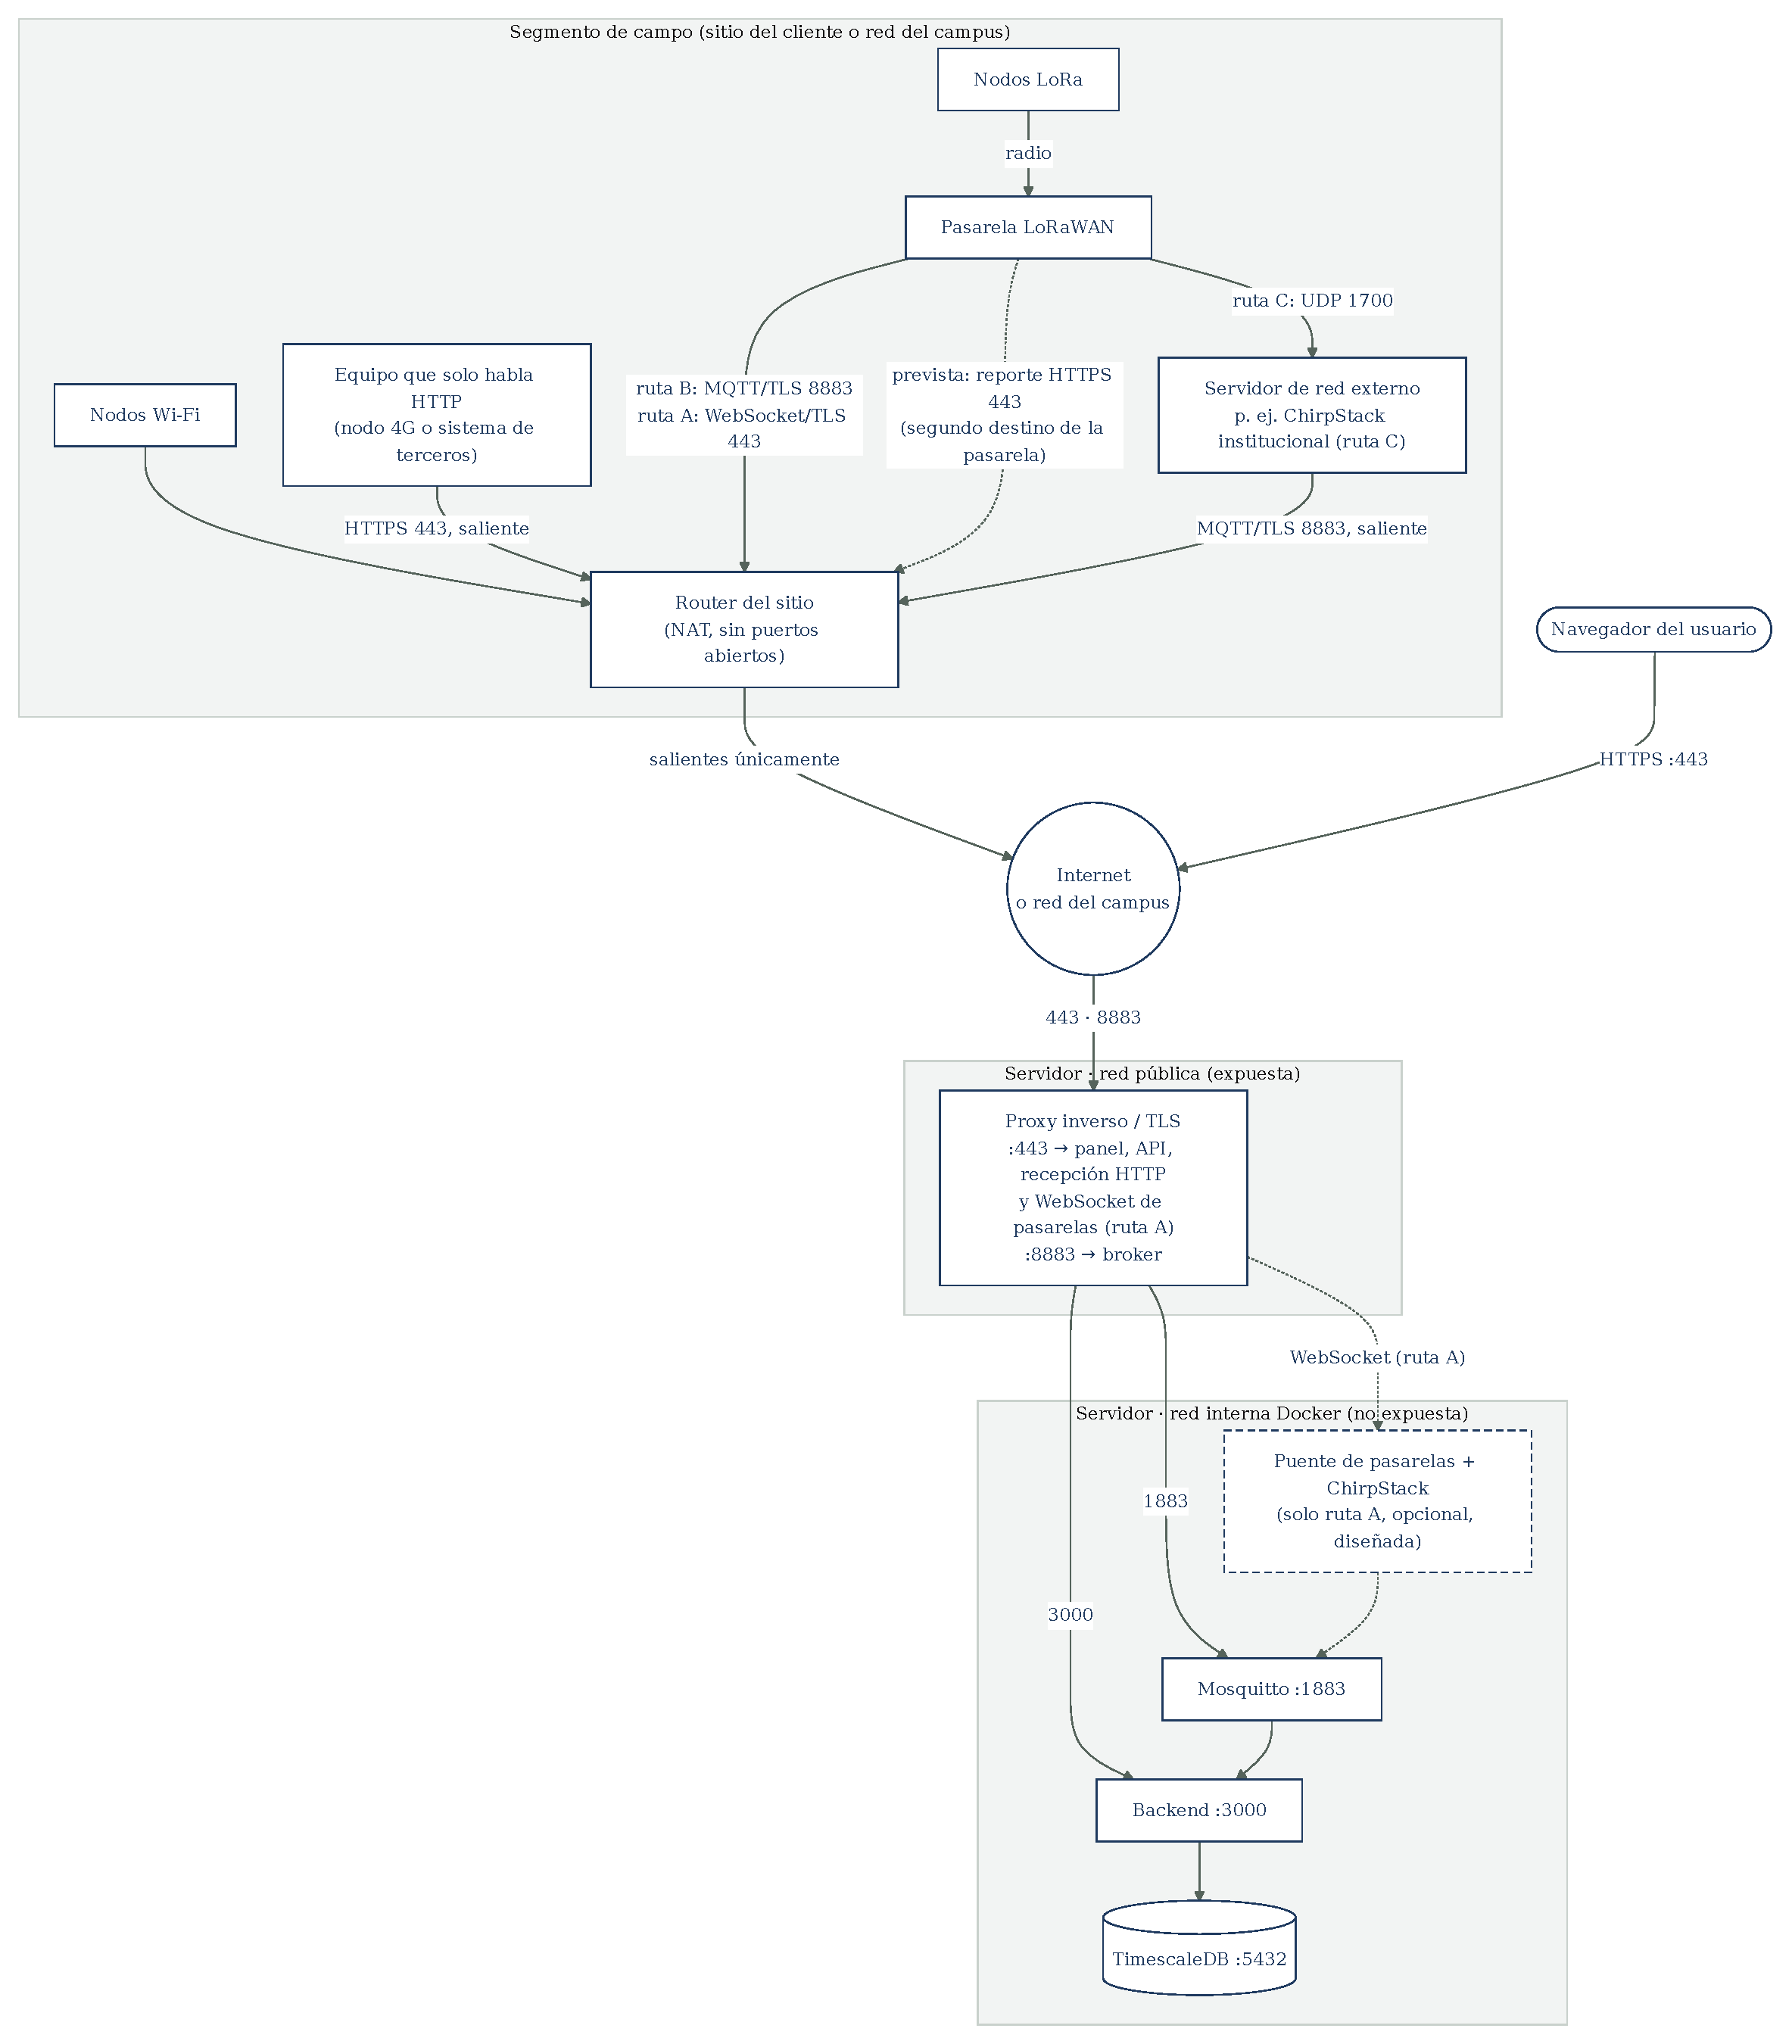
\includegraphics[width=\linewidth,height=0.85\textheight,keepaspectratio]{figuras/render/red.pdf}
\caption{Topología de red y segmentación. Los dispositivos del sitio solo abren conexiones \emph{salientes}: el router del cliente no necesita puertos abiertos ni configuración (RNF-10). Las tres vías de entrada (MQTT sobre TLS, HTTPS y, diseñada y punteada, WebSocket sobre TLS para la pasarela con \emph{Basics Station}) y el reporte HTTPS previsto de la pasarela cruzan el mismo router. En el servidor, únicamente el proxy con TLS es alcanzable desde Internet, siempre en 443 y 8883; broker, backend, base de datos y, si existe, ChirpStack (opcional, ruta A) viven en la red interna de los contenedores.}
\label{fig:red}
\end{figure}
